\documentclass{article}
\usepackage{graphicx}
\usepackage{url}
\usepackage{natbib}
\title{Big Literature in Climate Change}
\begin{document}
\maketitle
\begin{abstract}
Rapid increases in the number of studies published about climate change make a comprehensive assessment of the relevant literature ever more difficult. This in turn poses serious challenges for evidence-based decision making. In this paper we make the case that the challenges and opportunities presented by the explosion in relevant literature are akin to those presented by big data, and point to ways that machine learning techniques derived from big data could be applied to big literature.
\end{abstract}

\section{Introduction}
\begin{itemize}	

	\item Science policy, assessments - challenges of explosion.
    
	\item Big Literature in other sciences: \citet{Nunez-Mir2016}

	\item Canonical big data definition, 3 Vs + methods 

	\item Here, we estimate the size of the relevant literature and attempt to quantify it according to the dimensions above. This in itself is challenging due to the size of the data and requires new methods.  
\end{itemize}

\section{Estimating the Size of the Climate Literature}
% * <max.w.callaghan@gmail.com> 2017-03-23T12:44:52.581Z:
% 
% Include venn figure on WoS + Scopus & per year figure
% 
% ^.
Estimating the size of the relevant literature on climate change is not trivial. In \citet{minx2016learning}, we borrowed a query from \citet{Grieneisen2011} and showed how the number of references in IPCC reports had increased by x percent over 25 years, but reduced as a proportion of this estimate of relevant literature from x percent to y percent. In this paper we pointed out that this literature size estimate was very much a lower-bound estimate, neglecting as it does 
\begin{enumerate}
	\item literature, such as grey literature not published in peer reviewed journals 
    \item literature that is not included in the Web of Science (WoS) 
    \item literature that is not directly about climate change, but that is relevant to understanding the problem and its potential solutions, such as literature on international cooperation.
\end{enumerate}

In this paper, we attempt a more realistic estimate of the size of the literature on climate change by
\begin{enumerate}
	\item Carrying out the same query on Scopus, and combining the results with WoS
    \item Checking the references of the literature returned by the scopus query
\end{enumerate}

Figure 1 shows the 

\begin{figure}
%\includegraphics[width=\linewidth]{}
\caption{Union of Scopus and Web of Science results}
\end{figure}

\begin{figure}
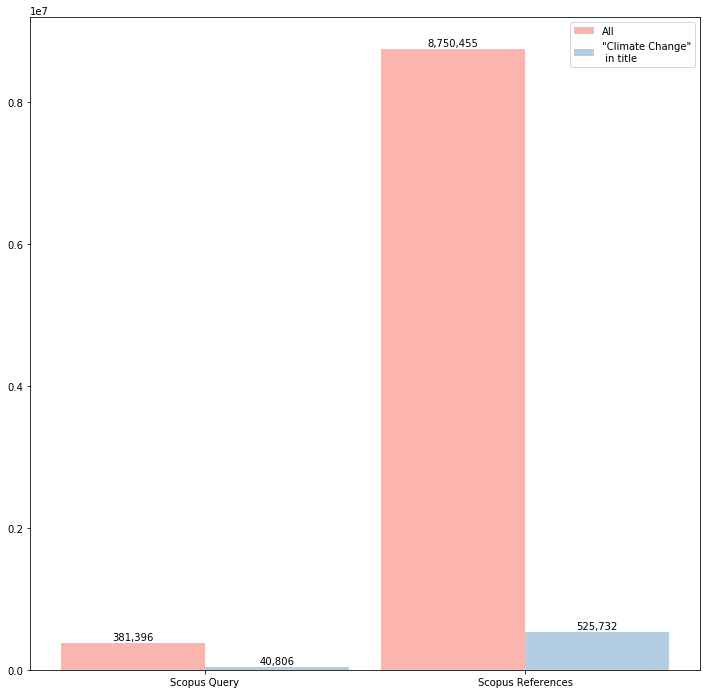
\includegraphics[width=\linewidth]{plots/scopus_docs_refs}
\caption{Number of papers retrieved from scopus, and the references contained within them}
\end{figure}


% * <max.w.callaghan@gmail.com> 2017-03-28T08:07:26.243Z:
% 
% Check for climate change in IPCC reference titles
% 
% ^.

\subsection{The 3 Vs}
\subsubsection*{Volume}
\subsubsection*{Variety}

\bibliography{Mendeley.bib}
\bibliographystyle{apalike}

\end{document}